\documentclass[uplatex, a4paper,twocolumn, 14pt]{jsarticle}

\usepackage{cite} % bibtex用パッケージ
\usepackage{amsmath} % 米国数学会パッケージ, 数式表現を強化する
\usepackage{abstract} % abstract作成用拡張パッケージ
\usepackage{authblk} % titleに所属を表示できるようになる
\usepackage[dvipdfmx]{graphicx} % 図の挿入
\usepackage[top=1.5cm,bottom=2cm,left=2cm,right=2cm]{geometry} % 余白調整
\usepackage{titlesec} % 見出し変更パッケージ
\usepackage{url} % urlに専用フォントスタイルとリンク追加
\usepackage[dvipdfmx]{hyperref} % ハイパーリンク生成
\usepackage{pxjahyper} % ハイパーリンク生成
\usepackage{lmodern}  % Latine Modern 欧文フォントの見栄えを安定化
\usepackage{secdot} % sectionのピリオドをカスタマイズ
\usepackage{listings} % コードブロック
% コードブロックの設定
\renewcommand{\lstlistingname}{Program}
\lstset{
  basicstyle={\ttfamily},
  identifierstyle={\small},
  commentstyle={\smallitshape},
  keywordstyle={\small\bfseries},
  ndkeywordstyle={\small},
  stringstyle={\small\ttfamily},
  breaklines=true,
  columns=[l]{fullflexible},
  numbers=left,
  xrightmargin=0zw,
  xleftmargin=3zw,
  numberstyle={\scriptsize},
  stepnumber=1,
  numbersep=1zw,
  lineskip=-0.5ex
}

% 著者表示をきれいに
\renewcommand\Authsep{\quad}
\renewcommand\Authand{\quad}
\renewcommand\Authands{\quad}

\begin{document}
% タイトル定義
\title{ここにタイトルを書く}
% % 著者(単独)
% \author{国立太郎}
% % 所属(単独)
% \affil{某国立大学}
% 著者(複数人)
\author[1]{国立太郎}
\author[2]{私立一郎}
\author[1]{国立次郎}
% 所属(複数人)
\affil[1]{某国立大学}
\affil[2]{某私立大学}
\date{} %日付非表示

% 概要
\twocolumn[
    \maketitle % タイトルを表示
    \begin{abstract}
        {\normalsize
            イエネコは、肉食性の小型哺乳類である。
            リビアヤマネコが家畜化した種のことを指し、通称として``猫''と呼ばれる。
            ペットとして人に人気があり、その人気から品種は約60種が確認されている。
            
            本論文ではこの生態と、LaTeXの書き方を示し、論文作成の際のテンプレートになることを目的とする。
            \par
        }
    \end{abstract}
    \vspace{1cm}%下との間隔を少し取る。
]




\section{文章}

ここの文章を書き直すことで、本文を書くことができる。
の本文では改行は無視される。
したがって、この文は前2つの文と改行無しでつながって出力される。

段落を分けるには、改行を2つ挟むことでこのように段落分けができる。

\subsection{章立てとラベル付け \label{sec:aaa}}

\verb|\section{節名}|, \verb|\subsection{小節名}|, \verb|\subsubsection{小々節名}|と書くことで節、小節、小々節を設定できる。

また、\verb|\section{節名 \label{sec:aaa}}|などと書くことで、\verb|sec:aaa|という名前でラベル付けする事ができる。
付けたラベルは\verb|\ref{sec:aaa}|などと書くことで、「\ref{sec:aaa}節」のように動的に節番号を取得することができる。
加えて、図番号や式番号にもラベル付けを行うことができる。
詳細は\ref{sec:graph}節, \ref{sec:equation}節で解説する。

\subsection{フッターの設定}
このように\footnote{aaa}書くことでフッターを設定できる。


\section{図と表}

\subsection{図 \label{sec:graph}}

このように書くことで、図を挿入できる。
\verb|graphics/cat.jpg|を差し替えることでファイルパスを変更できる。
大きさの調整、キャプションの入力、ラベルの設定ができる。
設定したラベルは「図\ref{graph:cat}」のように引用することができる。

\begin{figure}[tbh]
    \begin{center}
        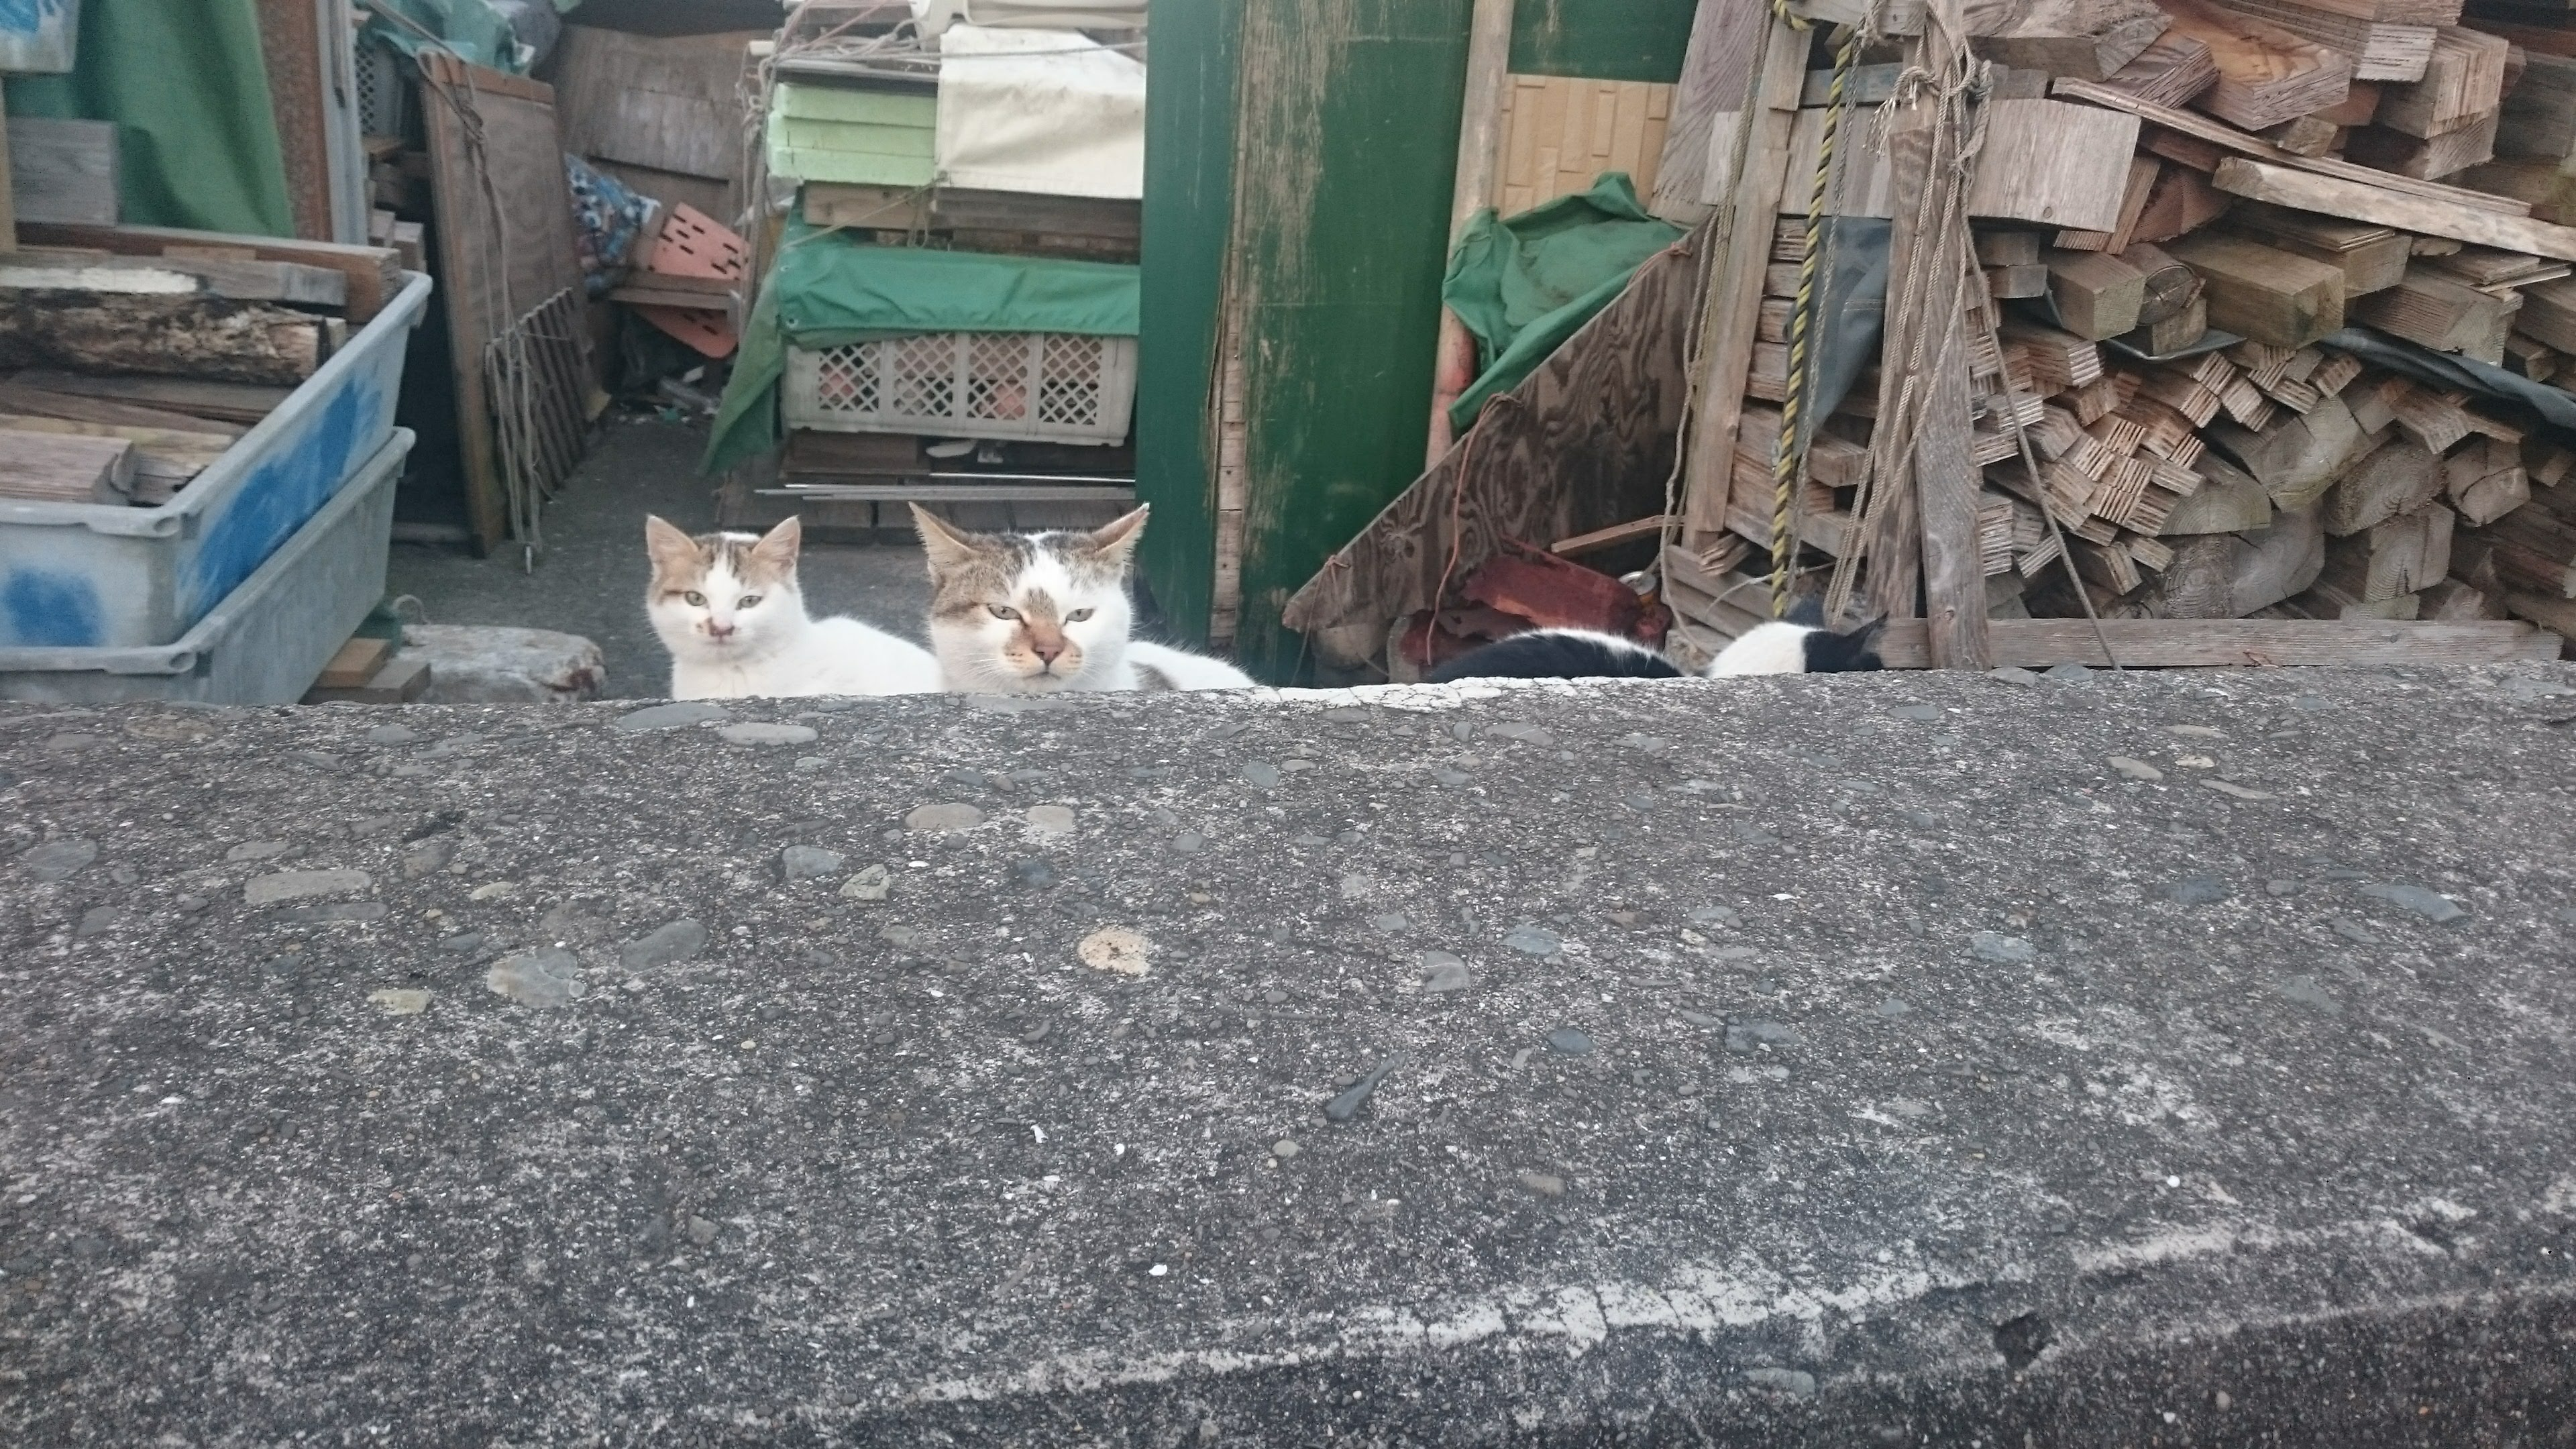
\includegraphics[width=8cm]{graphics/cat.jpg}
        \caption{
            地元を歩いていたときに見かけた猫。
        }
        \label{graph:cat}
    \end{center}
\end{figure}

また、図\ref{graph:cat_curve}のようにpdfファイルを読み込むことが可能である。
グラフを表示するときには、pngやjpgといったラスタ形式より、pdfやepsといったベクタ形式を利用するのが好ましい。

\begin{figure}[tbh]
    \begin{center}
        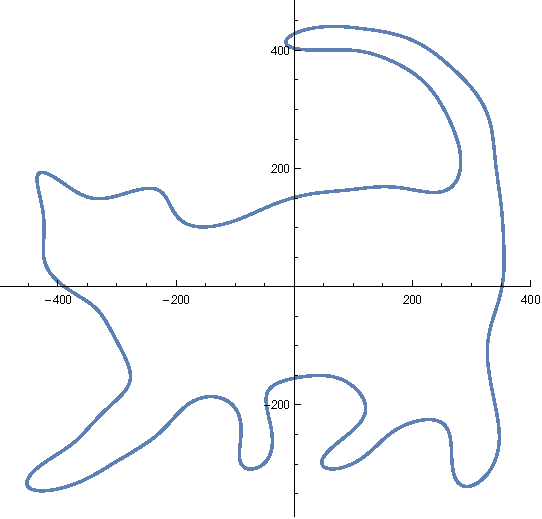
\includegraphics[width=6cm]{graphics/cat_curve.pdf}
        \caption{
            cat curve.
        }
        \label{graph:cat_curve}
    \end{center}
\end{figure}

\subsection{表}
次のように書くと、猫の生態を表で表せる。
\lstinline{|c|r}の部分を編集すると、区切りの線や中央・左右揃えを設定できる。

\begin{table}[tbh]
    \begin{center}
        \begin{tabular}{|c|r}
            体温 & 38.6 °C \\
            心拍数 & 120–140 毎分間の拍動の数 \\
            呼吸数 & 16–40 毎分呼吸
        \end{tabular}
        \caption{猫の生態\cite{kahn2007merck}}
        \label{tab:table-name}
    \end{center}
\end{table}

\subsection{プログラムコード}

\lstinline{print "Hello World"} のように書くと文中にプログラムコードを表示できる。
また、次のプログラム\ref{fuga}のように書くと、複数行のプログラムコードを表示できる。
オプション \lstinline{[caption=hoge,label=fuga]} の有無は任意。

\begin{lstlisting}[caption=hoge,label=fuga]
    void hello(){
        printf("Hello world!");
    }
\end{lstlisting}

\subsection{URLの表示}
\url{https://www.google.com/}のように書くとハイパーリンク付きURLを表示できる。
また\href{https://www.bing.com/}{このように}書くことで文章にURLのリンクを付けることもできる。

\section{引用論文}

\LaTeX ではBibTeXという機能で参考資料を管理できる。
この機能を用いることで、一般的な文章作成ソフトでは煩雑な参考文献の管理を簡単かつ機能的にできる。
この節では、BibTeXの設定方法について述べる。

\subsection{bibファイルの設定}
\lstinline{.tex}ファイルと同一の階層に\lstinline{.bib}ファイルを作成する。
\lstinline{.bib}ファイルは参考文献のリストを書いていく。
以下は\lstinline{.bib}ファイルに書く内容の一例である。

\begin{lstlisting}
@article{einstein1935can,
  title     = {Can quantum-mechanical description of physical reality be considered complete?},
  author    = {Einstein, Albert and Podolsky, Boris and Rosen, Nathan},
  journal   = {Physical review},
  volume    = {47},
  number    = {10},
  pages     = {777},
  year      = {1935},
  publisher = {APS}
}
\end{lstlisting}

\verb+@article{...}+ で囲まれたもの1つで、1つの文献を管理する。
論文以外の文献の種類を扱いたい場合、\lstinline{@article}以外の設定をすれば良い。
BiBTeXで扱える文献の種類は、\href{https://ja.wikipedia.org/wiki/BibTeX#%E3%82%A8%E3%83%B3%E3%83%88%E3%83%AA%E7%A8%AE%E5%88%A5}{Wikipedia}が参考になる。

文献の詳細は \verb+@article{...}+ の内側に書かれた各パラメータに記述する。
書き方については同じく、\href{https://ja.wikipedia.org/wiki/BibTeX#%E6%9B%B8%E8%AA%8C%E6%83%85%E5%A0%B1%E3%83%95%E3%82%A1%E3%82%A4%E3%83%AB}{Wikipedia}が参考になる。

また、論文検索サービス『Google Scholar\footnote{\url{https://scholar.google.com/}}』はBibTeXをサポートしている。
この機能を利用することで、知りたい論文を手早く\lstinline{.bib}ファイルに取り込める。
検索結果の下側にある引用符マーク(\lstinline{"})をクリックし、そこからBibTeXを選べば、BibTeXにそのままコピー&ペーストできるデータを入手できる。

\subsection{参考文献の一覧を表示}
\lstinline{.tex}ファイルの最後( \verb+\end{document}+ の一つ前の行あたり)に以下のように書くと、本文中に引用した文献の一覧が表示される。
なお、本文中で文献を引用する方法は\ref{sec:call_bib}節で述べる。

\begin{lstlisting}
    \bibliography{ファイル名.bib}{}
    \bibliographystyle{junsrt}
\end{lstlisting}

\verb+\bibliographystyle{...}+で表示スタイルを指定できる。
\verb+\bibliographystyle{junsrt}+ならば、引用の早い順で表示される。
詳細は\href{https://ja.overleaf.com/learn/latex/Bibtex_bibliography_styles}{こちらのサイト}を参考にするとよい。

\subsection{参考文献の呼び出し \label{sec:call_bib}}
\lstinline{.bib}ファイルに登録した参考文献を引用したい場合は、文中で\verb+\cite{einstein1935can}+などと書けば、このように表示される\cite{einstein1935can}。
\verb+\cite{...}+ で指定する名前は \lstinline{.bib} ファイルの各文献1行目にある名前で識別している。

\begin{lstlisting}
    @article{einstein1935can,  ←これ
      title     = {Can quantum-mechanical description of physical reality be considered complete?},
\end{lstlisting}

\section{数式 \label{sec:equation}}

LaTeXは科学論文に用いられているという背景から、数式の表示には豊富な機能を持っている。
式(\ref{eq:example1}), (\ref{eq:example2})はその一例である。
\begin{equation} \label{eq:example1}
    e^{i \theta} = \cos{\theta} + i \sin{\theta}
\end{equation}
\begin{equation} \label{eq:example2}
    \cos{x} = 1 - \frac{x^2}{2!} + \frac{x^4}{4!} - \cdots
\end{equation}

% bibファイル読み込み & Reference表示
\bibliography{reference.bib}{}
\bibliographystyle{junsrt}

\end{document}